\documentclass[tikz]{standalone}
\usetikzlibrary{math,shapes.geometric,calc,positioning}

\begin{document}
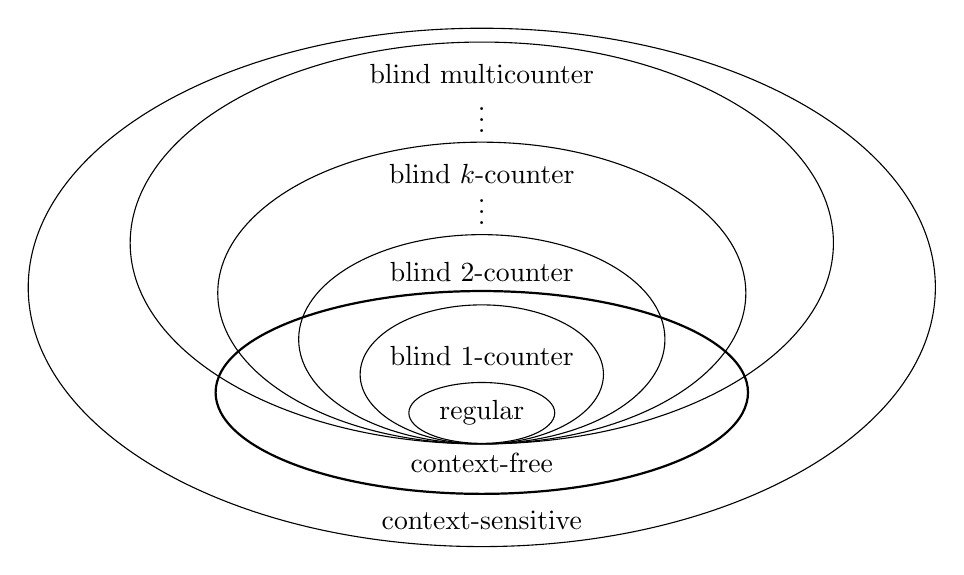
\begin{tikzpicture}[xscale=3.5,yscale=2]
	
	\coordinate (zero) at (0,0);
	
	\node [ellipse,above=0pt of zero,draw] (regular) {regular};
	\coordinate (regular-top) at ($(regular.north)$);
	
	%%%%%%%%%%%%%%%%%%%%%%%%%%%%%%%%%%%%%%%%%%%%%%%%%%%%%%
	
	\node [above=0.25em of regular-top] (1-counter-text) {blind 1-counter};
	
	\draw [inner sep=0pt,outer sep=0pt,draw] let
	\p1=($(1-counter-text.north)$),
	\p2=($(1-counter-text.east)$),
	\n1={\x2/sin(180 - 2*atan2(\y1,\x2))}
	in
	(0,\n1) circle (\n1);
	%
	\path let
	\p1=($(1-counter-text.north)$),
	\p2=($(1-counter-text.east)$),
	\n1={\x2/sin(180 - 2*atan2(\y1,\x2))}
	in coordinate
	(1-counter-top) at (0,2*\n1);
	
	%%%%%%%%%%%%%%%%%%%%%%%%%%%%%%%%%%%%%%%%%%%%%%%%%%%%%%
	
	\node [below=0pt of zero] (context-free-text) {context-free};
	
	\draw [inner sep=0pt,outer sep=0pt,draw,thick] let
	\p1=($(1-counter-top)$),
	\p2=($(context-free-text.east)$),
	\p3=($(context-free-text.south)$),
	\p0=($(\x2,\y1-\y3+0.25em)$),
	\n1={\x0/sin(180 - 2*atan2(\x0,\y0))}
	in
	($(0,\y1-\n1+0.25em)$) ellipse (1.5*\n1 and \n1);
	%
	\path let
	\p1=($(1-counter-top)$),
	\p2=($(context-free-text.east)$),
	\p3=($(context-free-text.south)$),
	\p0=($(\x2,\y1-\y3+0.25em)$),
	\n1={\x0/sin(180 - 2*atan2(\x0,\y0))}
	in coordinate
	(context-free-bottom) at (0,\y1-2*\n1+0.25em);
	
	%%%%%%%%%%%%%%%%%%%%%%%%%%%%%%%%%%%%%%%%%%%%%%%%%%%%%%
	
	\node [above=0.5em of 1-counter-top] (2-counter-text) {blind 2-counter};
	
	\draw [inner sep=0pt,outer sep=0pt,draw] let
	\p1=($(2-counter-text.north)$),
	\p2=($(2-counter-text.east)$),
	\n1={\x2/sin(180-2*atan2(\x2,\y1))}
	in
	(0,\n1) circle (\n1);
	%
	\path let
	\p1=($(2-counter-text.north)$),
	\p2=($(2-counter-text.east)$),
	\n1={\x2/sin(180-2*atan2(\x2,\y1))}
	in coordinate
	(2-counter-top-real) at (0,2*\n1);
	
	%%%%%%%%%%%%%%%%%%%%%%%%%%%%%%%%%%%%%%%%%%%%%%%%%%%%%%
	
	\node [above=0em of 2-counter-top-real] (2-counter-top) {$\makeatletter
		\vbox{
			\baselineskip4\p@\lineskiplimit\z@
			\kern-\p@
			\hbox{.}\hbox{.}\hbox{.}
		}
		\makeatother$};
	
	%%%%%%%%%%%%%%%%%%%%%%%%%%%%%%%%%%%%%%%%%%%%%%%%%%%%%%
	
	\node [above=0em of 2-counter-top] (3-counter-text) {blind $k$-counter};
	
	\draw [inner sep=0pt,outer sep=0pt,draw] let
	\p1=($(3-counter-text.north)$),
	\p2=($(3-counter-text.east)$),
	\n1={\x2/sin(180-2*atan2(\x2,\y1))}
	in
	(0,\n1) circle (\n1);
	%
	\path let
	\p1=($(3-counter-text.north)$),
	\p2=($(3-counter-text.east)$),
	\n1={\x2/sin(180-2*atan2(\x2,\y1))}
	in coordinate
	(3-counter-top) at (0,2*\n1);
	
	%%%%%%%%%%%%%%%%%%%%%%%%%%%%%%%%%%%%%%%%%%%%%%%%%%%%%%
	
	\node [above=0em of 3-counter-top] (dots) {$\makeatletter
		\vbox{
			\baselineskip4\p@\lineskiplimit\z@
			\kern-\p@
			\hbox{.}\hbox{.}\hbox{.}
		}
		\makeatother$};
	
	%%%%%%%%%%%%%%%%%%%%%%%%%%%%%%%%%%%%%%%%%%%%%%%%%%%%%%
	
	\node [above=0.25em of dots] (k-counter-text) {blind multicounter};
	
	\draw [inner sep=0pt,outer sep=0pt,draw] let
	\p1=($(k-counter-text.north)$),
	\p2=($(k-counter-text.east)$),
	\n1={\x2/sin(180-2*atan2(\x2,\y1))}
	in
	(0,\n1) circle (\n1);
	%
	\path let
	\p1=($(k-counter-text.north)$),
	\p2=($(k-counter-text.east)$),
	\n1={\x2/sin(180-2*atan2(\x2,\y1))}
	in coordinate
	(k-counter-top) at (0,2*\n1);
	
	%%%%%%%%%%%%%%%%%%%%%%%%%%%%%%%%%%%%%%%%%%%%%%%%%%%%%%
	
	\node [below=0.25em of context-free-bottom] (context-sentivite-text) {context-sensitive};
	
	\draw [inner sep=0pt,outer sep=0pt,draw] let
	\p1=($(k-counter-top)$),
	\p2=($(context-sentivite-text.east)$),
	\p3=($(context-sentivite-text.south)$),
	\p0=($(\x2,\y1-\y3+0.25em)$),
	\n1={\x0/sin(180-2*atan2(\x0,\y0))}
	in
	($(0,\y1-\n1+0.25em)$) circle (\n1);
	
	%%%%%%%%%%%%%%%%%%%%%%%%%%%%%%%%%%%%%%%%%%%%%%%%%%%%%%
	
\end{tikzpicture}
\end{document}